% fig_signature.tex -- generated by signature/signature.py (figure step) from sig_auroc.csv; do not edit by hand.
\definecolor{fpV}{HTML}{D55E00}\definecolor{fpB}{HTML}{0072B2}%
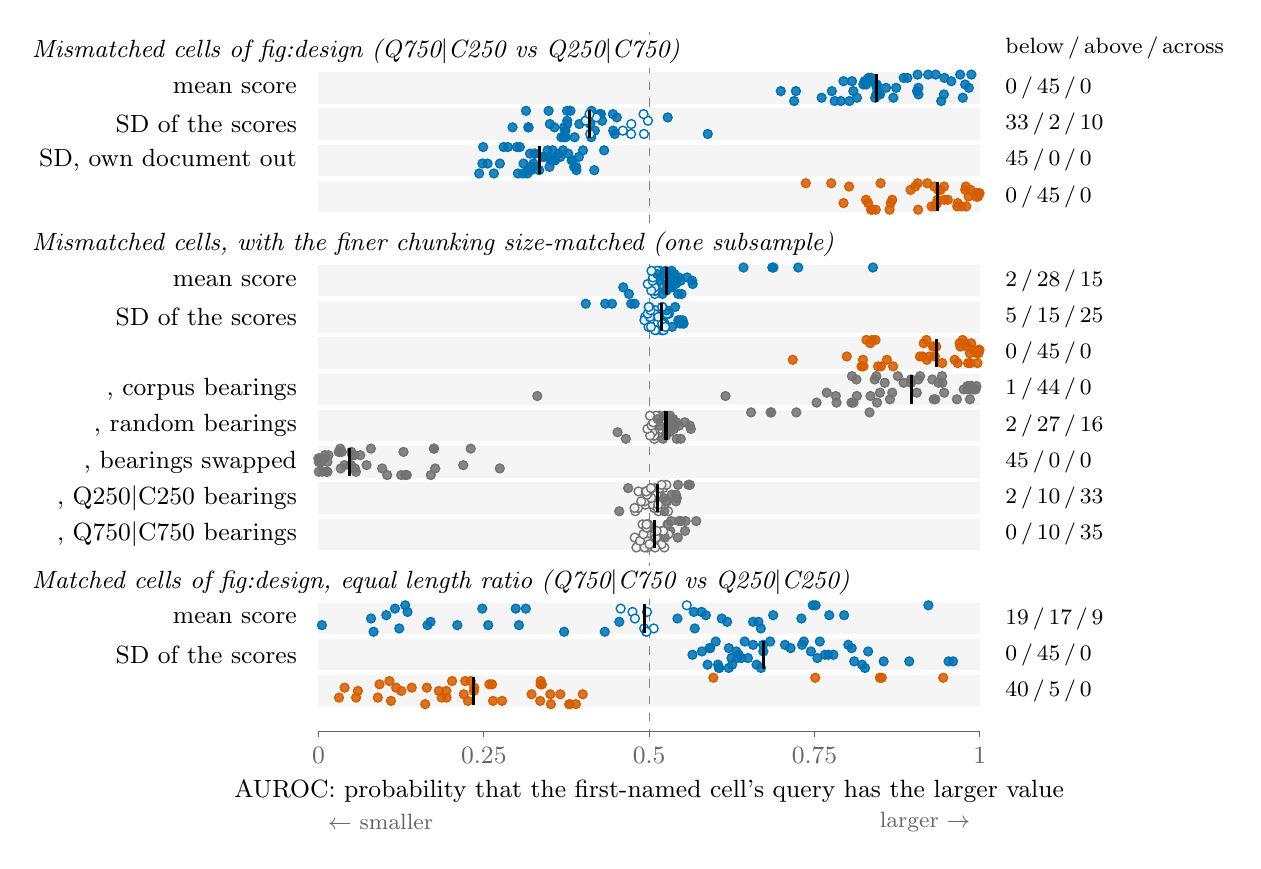
\begin{tikzpicture}[font=\small]
\fill[black!4] (0,-0.660) rectangle (8.400,-0.260);
\fill[black!4] (0,-1.120) rectangle (8.400,-0.720);
\fill[black!4] (0,-1.580) rectangle (8.400,-1.180);
\fill[black!4] (0,-2.040) rectangle (8.400,-1.640);
\fill[black!4] (0,-3.110) rectangle (8.400,-2.710);
\fill[black!4] (0,-3.570) rectangle (8.400,-3.170);
\fill[black!4] (0,-4.030) rectangle (8.400,-3.630);
\fill[black!4] (0,-4.490) rectangle (8.400,-4.090);
\fill[black!4] (0,-4.950) rectangle (8.400,-4.550);
\fill[black!4] (0,-5.410) rectangle (8.400,-5.010);
\fill[black!4] (0,-5.870) rectangle (8.400,-5.470);
\fill[black!4] (0,-6.330) rectangle (8.400,-5.930);
\fill[black!4] (0,-7.400) rectangle (8.400,-7.000);
\fill[black!4] (0,-7.860) rectangle (8.400,-7.460);
\fill[black!4] (0,-8.320) rectangle (8.400,-7.920);
\draw[black!50, dashed] (4.200,0.250) -- (4.200,-8.630);
\node[anchor=west, font=\small\itshape, fill=white, inner sep=1.5pt] at (-3.7,0.000) {Mismatched cells of \cref{fig:design} (Q750$|$C250 vs Q250$|$C750)};
\node[anchor=east] at (-0.15,-0.460) {mean score};
\path[fill=fpB, draw=fpB, line width=0.5pt, fill opacity=0.85] (6.743,-0.628) circle (1.6pt);
\path[fill=fpB, draw=fpB, line width=0.5pt, fill opacity=0.85] (7.301,-0.586) circle (1.6pt);
\path[fill=fpB, draw=fpB, line width=0.5pt, fill opacity=0.85] (7.620,-0.544) circle (1.6pt);
\path[fill=fpB, draw=fpB, line width=0.5pt, fill opacity=0.85] (5.872,-0.502) circle (1.6pt);
\path[fill=fpB, draw=fpB, line width=0.5pt, fill opacity=0.85] (7.619,-0.460) circle (1.6pt);
\path[fill=fpB, draw=fpB, line width=0.5pt, fill opacity=0.85] (7.091,-0.418) circle (1.6pt);
\path[fill=fpB, draw=fpB, line width=0.5pt, fill opacity=0.85] (6.935,-0.376) circle (1.6pt);
\path[fill=fpB, draw=fpB, line width=0.5pt, fill opacity=0.85] (7.432,-0.334) circle (1.6pt);
\path[fill=fpB, draw=fpB, line width=0.5pt, fill opacity=0.85] (8.150,-0.292) circle (1.6pt);
\path[fill=fpB, draw=fpB, line width=0.5pt, fill opacity=0.85] (6.633,-0.628) circle (1.6pt);
\path[fill=fpB, draw=fpB, line width=0.5pt, fill opacity=0.85] (6.390,-0.586) circle (1.6pt);
\path[fill=fpB, draw=fpB, line width=0.5pt, fill opacity=0.85] (7.113,-0.544) circle (1.6pt);
\path[fill=fpB, draw=fpB, line width=0.5pt, fill opacity=0.85] (6.064,-0.502) circle (1.6pt);
\path[fill=fpB, draw=fpB, line width=0.5pt, fill opacity=0.85] (7.337,-0.460) circle (1.6pt);
\path[fill=fpB, draw=fpB, line width=0.5pt, fill opacity=0.85] (7.077,-0.418) circle (1.6pt);
\path[fill=fpB, draw=fpB, line width=0.5pt, fill opacity=0.85] (6.776,-0.376) circle (1.6pt);
\path[fill=fpB, draw=fpB, line width=0.5pt, fill opacity=0.85] (6.986,-0.334) circle (1.6pt);
\path[fill=fpB, draw=fpB, line width=0.5pt, fill opacity=0.85] (7.839,-0.292) circle (1.6pt);
\path[fill=fpB, draw=fpB, line width=0.5pt, fill opacity=0.85] (6.556,-0.628) circle (1.6pt);
\path[fill=fpB, draw=fpB, line width=0.5pt, fill opacity=0.85] (7.070,-0.586) circle (1.6pt);
\path[fill=fpB, draw=fpB, line width=0.5pt, fill opacity=0.85] (7.132,-0.544) circle (1.6pt);
\path[fill=fpB, draw=fpB, line width=0.5pt, fill opacity=0.85] (6.520,-0.502) circle (1.6pt);
\path[fill=fpB, draw=fpB, line width=0.5pt, fill opacity=0.85] (7.208,-0.460) circle (1.6pt);
\path[fill=fpB, draw=fpB, line width=0.5pt, fill opacity=0.85] (6.954,-0.418) circle (1.6pt);
\path[fill=fpB, draw=fpB, line width=0.5pt, fill opacity=0.85] (6.954,-0.376) circle (1.6pt);
\path[fill=fpB, draw=fpB, line width=0.5pt, fill opacity=0.85] (7.479,-0.334) circle (1.6pt);
\path[fill=fpB, draw=fpB, line width=0.5pt, fill opacity=0.85] (7.743,-0.292) circle (1.6pt);
\path[fill=fpB, draw=fpB, line width=0.5pt, fill opacity=0.85] (6.041,-0.628) circle (1.6pt);
\path[fill=fpB, draw=fpB, line width=0.5pt, fill opacity=0.85] (6.839,-0.586) circle (1.6pt);
\path[fill=fpB, draw=fpB, line width=0.5pt, fill opacity=0.85] (7.084,-0.544) circle (1.6pt);
\path[fill=fpB, draw=fpB, line width=0.5pt, fill opacity=0.85] (6.793,-0.502) circle (1.6pt);
\path[fill=fpB, draw=fpB, line width=0.5pt, fill opacity=0.85] (7.091,-0.460) circle (1.6pt);
\path[fill=fpB, draw=fpB, line width=0.5pt, fill opacity=0.85] (6.920,-0.418) circle (1.6pt);
\path[fill=fpB, draw=fpB, line width=0.5pt, fill opacity=0.85] (6.668,-0.376) circle (1.6pt);
\path[fill=fpB, draw=fpB, line width=0.5pt, fill opacity=0.85] (7.021,-0.334) circle (1.6pt);
\path[fill=fpB, draw=fpB, line width=0.5pt, fill opacity=0.85] (7.609,-0.292) circle (1.6pt);
\path[fill=fpB, draw=fpB, line width=0.5pt, fill opacity=0.85] (7.909,-0.628) circle (1.6pt);
\path[fill=fpB, draw=fpB, line width=0.5pt, fill opacity=0.85] (8.183,-0.586) circle (1.6pt);
\path[fill=fpB, draw=fpB, line width=0.5pt, fill opacity=0.85] (7.943,-0.544) circle (1.6pt);
\path[fill=fpB, draw=fpB, line width=0.5pt, fill opacity=0.85] (7.602,-0.502) circle (1.6pt);
\path[fill=fpB, draw=fpB, line width=0.5pt, fill opacity=0.85] (8.260,-0.460) circle (1.6pt);
\path[fill=fpB, draw=fpB, line width=0.5pt, fill opacity=0.85] (8.213,-0.418) circle (1.6pt);
\path[fill=fpB, draw=fpB, line width=0.5pt, fill opacity=0.85] (8.037,-0.376) circle (1.6pt);
\path[fill=fpB, draw=fpB, line width=0.5pt, fill opacity=0.85] (7.950,-0.334) circle (1.6pt);
\path[fill=fpB, draw=fpB, line width=0.5pt, fill opacity=0.85] (8.292,-0.292) circle (1.6pt);
\draw[black, line width=1.1pt] (7.091,-0.640) -- (7.091,-0.280);
\node[anchor=west, font=\footnotesize] at (8.600,-0.460) {0\,/\,45\,/\,0};
\node[anchor=east] at (-0.15,-0.920) {SD of the scores};
\path[fill=fpB, draw=fpB, line width=0.5pt, fill opacity=0.85] (3.464,-1.088) circle (1.6pt);
\path[fill=fpB, draw=fpB, line width=0.5pt, fill opacity=0.85] (4.944,-1.046) circle (1.6pt);
\path[fill=fpB, draw=fpB, line width=0.5pt, fill opacity=0.85] (3.131,-1.004) circle (1.6pt);
\path[fill=fpB, draw=fpB, line width=0.5pt, fill opacity=0.85] (2.667,-0.962) circle (1.6pt);
\path[fill=fpB, draw=fpB, line width=0.5pt, fill opacity=0.85] (3.313,-0.920) circle (1.6pt);
\path[fill=white, draw=fpB, line width=0.5pt, fill opacity=0.85] (4.185,-0.878) circle (1.6pt);
\path[fill=fpB, draw=fpB, line width=0.5pt, fill opacity=0.85] (4.435,-0.836) circle (1.6pt);
\path[fill=white, draw=fpB, line width=0.5pt, fill opacity=0.85] (4.129,-0.794) circle (1.6pt);
\path[fill=fpB, draw=fpB, line width=0.5pt, fill opacity=0.85] (3.468,-0.752) circle (1.6pt);
\path[fill=fpB, draw=fpB, line width=0.5pt, fill opacity=0.85] (3.253,-1.088) circle (1.6pt);
\path[fill=fpB, draw=fpB, line width=0.5pt, fill opacity=0.85] (3.763,-1.046) circle (1.6pt);
\path[fill=fpB, draw=fpB, line width=0.5pt, fill opacity=0.85] (3.137,-1.004) circle (1.6pt);
\path[fill=fpB, draw=fpB, line width=0.5pt, fill opacity=0.85] (2.997,-0.962) circle (1.6pt);
\path[fill=fpB, draw=fpB, line width=0.5pt, fill opacity=0.85] (2.939,-0.920) circle (1.6pt);
\path[fill=fpB, draw=fpB, line width=0.5pt, fill opacity=0.85] (3.159,-0.878) circle (1.6pt);
\path[fill=fpB, draw=fpB, line width=0.5pt, fill opacity=0.85] (3.436,-0.836) circle (1.6pt);
\path[fill=fpB, draw=fpB, line width=0.5pt, fill opacity=0.85] (3.587,-0.794) circle (1.6pt);
\path[fill=fpB, draw=fpB, line width=0.5pt, fill opacity=0.85] (2.636,-0.752) circle (1.6pt);
\path[fill=fpB, draw=fpB, line width=0.5pt, fill opacity=0.85] (3.085,-1.088) circle (1.6pt);
\path[fill=white, draw=fpB, line width=0.5pt, fill opacity=0.85] (4.134,-1.046) circle (1.6pt);
\path[fill=fpB, draw=fpB, line width=0.5pt, fill opacity=0.85] (3.510,-1.004) circle (1.6pt);
\path[fill=fpB, draw=fpB, line width=0.5pt, fill opacity=0.85] (2.667,-0.962) circle (1.6pt);
\path[fill=fpB, draw=fpB, line width=0.5pt, fill opacity=0.85] (3.158,-0.920) circle (1.6pt);
\path[fill=fpB, draw=fpB, line width=0.5pt, fill opacity=0.85] (3.391,-0.878) circle (1.6pt);
\path[fill=fpB, draw=fpB, line width=0.5pt, fill opacity=0.85] (3.511,-0.836) circle (1.6pt);
\path[fill=fpB, draw=fpB, line width=0.5pt, fill opacity=0.85] (3.567,-0.794) circle (1.6pt);
\path[fill=fpB, draw=fpB, line width=0.5pt, fill opacity=0.85] (3.157,-0.752) circle (1.6pt);
\path[fill=fpB, draw=fpB, line width=0.5pt, fill opacity=0.85] (3.116,-1.088) circle (1.6pt);
\path[fill=white, draw=fpB, line width=0.5pt, fill opacity=0.85] (3.971,-1.046) circle (1.6pt);
\path[fill=fpB, draw=fpB, line width=0.5pt, fill opacity=0.85] (3.743,-1.004) circle (1.6pt);
\path[fill=fpB, draw=fpB, line width=0.5pt, fill opacity=0.85] (2.465,-0.962) circle (1.6pt);
\path[fill=fpB, draw=fpB, line width=0.5pt, fill opacity=0.85] (3.452,-0.920) circle (1.6pt);
\path[fill=fpB, draw=fpB, line width=0.5pt, fill opacity=0.85] (3.602,-0.878) circle (1.6pt);
\path[fill=fpB, draw=fpB, line width=0.5pt, fill opacity=0.85] (3.789,-0.836) circle (1.6pt);
\path[fill=fpB, draw=fpB, line width=0.5pt, fill opacity=0.85] (3.740,-0.794) circle (1.6pt);
\path[fill=fpB, draw=fpB, line width=0.5pt, fill opacity=0.85] (3.200,-0.752) circle (1.6pt);
\path[fill=fpB, draw=fpB, line width=0.5pt, fill opacity=0.85] (3.140,-1.088) circle (1.6pt);
\path[fill=white, draw=fpB, line width=0.5pt, fill opacity=0.85] (3.451,-1.046) circle (1.6pt);
\path[fill=white, draw=fpB, line width=0.5pt, fill opacity=0.85] (3.866,-1.004) circle (1.6pt);
\path[fill=fpB, draw=fpB, line width=0.5pt, fill opacity=0.85] (3.119,-0.962) circle (1.6pt);
\path[fill=white, draw=fpB, line width=0.5pt, fill opacity=0.85] (3.973,-0.920) circle (1.6pt);
\path[fill=white, draw=fpB, line width=0.5pt, fill opacity=0.85] (3.394,-0.878) circle (1.6pt);
\path[fill=white, draw=fpB, line width=0.5pt, fill opacity=0.85] (3.529,-0.836) circle (1.6pt);
\path[fill=white, draw=fpB, line width=0.5pt, fill opacity=0.85] (3.442,-0.794) circle (1.6pt);
\path[fill=fpB, draw=fpB, line width=0.5pt, fill opacity=0.85] (2.923,-0.752) circle (1.6pt);
\draw[black, line width=1.1pt] (3.442,-1.100) -- (3.442,-0.740);
\node[anchor=west, font=\footnotesize] at (8.600,-0.920) {33\,/\,2\,/\,10};
\node[anchor=east] at (-0.15,-1.380) {SD, own document out};
\path[fill=fpB, draw=fpB, line width=0.5pt, fill opacity=0.85] (2.653,-1.548) circle (1.6pt);
\path[fill=fpB, draw=fpB, line width=0.5pt, fill opacity=0.85] (3.503,-1.506) circle (1.6pt);
\path[fill=fpB, draw=fpB, line width=0.5pt, fill opacity=0.85] (3.273,-1.464) circle (1.6pt);
\path[fill=fpB, draw=fpB, line width=0.5pt, fill opacity=0.85] (2.082,-1.422) circle (1.6pt);
\path[fill=fpB, draw=fpB, line width=0.5pt, fill opacity=0.85] (3.217,-1.380) circle (1.6pt);
\path[fill=fpB, draw=fpB, line width=0.5pt, fill opacity=0.85] (3.307,-1.338) circle (1.6pt);
\path[fill=fpB, draw=fpB, line width=0.5pt, fill opacity=0.85] (3.047,-1.296) circle (1.6pt);
\path[fill=fpB, draw=fpB, line width=0.5pt, fill opacity=0.85] (3.628,-1.254) circle (1.6pt);
\path[fill=fpB, draw=fpB, line width=0.5pt, fill opacity=0.85] (2.520,-1.212) circle (1.6pt);
\path[fill=fpB, draw=fpB, line width=0.5pt, fill opacity=0.85] (2.597,-1.548) circle (1.6pt);
\path[fill=fpB, draw=fpB, line width=0.5pt, fill opacity=0.85] (2.699,-1.506) circle (1.6pt);
\path[fill=fpB, draw=fpB, line width=0.5pt, fill opacity=0.85] (2.724,-1.464) circle (1.6pt);
\path[fill=fpB, draw=fpB, line width=0.5pt, fill opacity=0.85] (2.605,-1.422) circle (1.6pt);
\path[fill=fpB, draw=fpB, line width=0.5pt, fill opacity=0.85] (3.004,-1.380) circle (1.6pt);
\path[fill=fpB, draw=fpB, line width=0.5pt, fill opacity=0.85] (2.849,-1.338) circle (1.6pt);
\path[fill=fpB, draw=fpB, line width=0.5pt, fill opacity=0.85] (2.686,-1.296) circle (1.6pt);
\path[fill=fpB, draw=fpB, line width=0.5pt, fill opacity=0.85] (2.974,-1.254) circle (1.6pt);
\path[fill=fpB, draw=fpB, line width=0.5pt, fill opacity=0.85] (2.352,-1.212) circle (1.6pt);
\path[fill=fpB, draw=fpB, line width=0.5pt, fill opacity=0.85] (2.533,-1.548) circle (1.6pt);
\path[fill=fpB, draw=fpB, line width=0.5pt, fill opacity=0.85] (3.276,-1.506) circle (1.6pt);
\path[fill=fpB, draw=fpB, line width=0.5pt, fill opacity=0.85] (3.247,-1.464) circle (1.6pt);
\path[fill=fpB, draw=fpB, line width=0.5pt, fill opacity=0.85] (2.148,-1.422) circle (1.6pt);
\path[fill=fpB, draw=fpB, line width=0.5pt, fill opacity=0.85] (3.219,-1.380) circle (1.6pt);
\path[fill=fpB, draw=fpB, line width=0.5pt, fill opacity=0.85] (3.071,-1.338) circle (1.6pt);
\path[fill=fpB, draw=fpB, line width=0.5pt, fill opacity=0.85] (3.172,-1.296) circle (1.6pt);
\path[fill=fpB, draw=fpB, line width=0.5pt, fill opacity=0.85] (3.360,-1.254) circle (1.6pt);
\path[fill=fpB, draw=fpB, line width=0.5pt, fill opacity=0.85] (2.405,-1.212) circle (1.6pt);
\path[fill=fpB, draw=fpB, line width=0.5pt, fill opacity=0.85] (2.041,-1.548) circle (1.6pt);
\path[fill=fpB, draw=fpB, line width=0.5pt, fill opacity=0.85] (2.804,-1.506) circle (1.6pt);
\path[fill=fpB, draw=fpB, line width=0.5pt, fill opacity=0.85] (2.691,-1.464) circle (1.6pt);
\path[fill=fpB, draw=fpB, line width=0.5pt, fill opacity=0.85] (2.304,-1.422) circle (1.6pt);
\path[fill=fpB, draw=fpB, line width=0.5pt, fill opacity=0.85] (2.948,-1.380) circle (1.6pt);
\path[fill=fpB, draw=fpB, line width=0.5pt, fill opacity=0.85] (2.927,-1.338) circle (1.6pt);
\path[fill=fpB, draw=fpB, line width=0.5pt, fill opacity=0.85] (2.754,-1.296) circle (1.6pt);
\path[fill=fpB, draw=fpB, line width=0.5pt, fill opacity=0.85] (2.910,-1.254) circle (1.6pt);
\path[fill=fpB, draw=fpB, line width=0.5pt, fill opacity=0.85] (2.092,-1.212) circle (1.6pt);
\path[fill=fpB, draw=fpB, line width=0.5pt, fill opacity=0.85] (2.228,-1.548) circle (1.6pt);
\path[fill=fpB, draw=fpB, line width=0.5pt, fill opacity=0.85] (2.661,-1.506) circle (1.6pt);
\path[fill=fpB, draw=fpB, line width=0.5pt, fill opacity=0.85] (2.934,-1.464) circle (1.6pt);
\path[fill=fpB, draw=fpB, line width=0.5pt, fill opacity=0.85] (2.730,-1.422) circle (1.6pt);
\path[fill=fpB, draw=fpB, line width=0.5pt, fill opacity=0.85] (3.005,-1.380) circle (1.6pt);
\path[fill=fpB, draw=fpB, line width=0.5pt, fill opacity=0.85] (2.864,-1.338) circle (1.6pt);
\path[fill=fpB, draw=fpB, line width=0.5pt, fill opacity=0.85] (2.741,-1.296) circle (1.6pt);
\path[fill=fpB, draw=fpB, line width=0.5pt, fill opacity=0.85] (3.106,-1.254) circle (1.6pt);
\path[fill=fpB, draw=fpB, line width=0.5pt, fill opacity=0.85] (2.558,-1.212) circle (1.6pt);
\draw[black, line width=1.1pt] (2.804,-1.560) -- (2.804,-1.200);
\node[anchor=west, font=\footnotesize] at (8.600,-1.380) {45\,/\,0\,/\,0};
\node[anchor=east] at (-0.15,-1.840) {$\Wone$};
\path[fill=fpV, draw=fpV, line width=0.5pt, fill opacity=0.85] (7.036,-2.008) circle (1.6pt);
\path[fill=fpV, draw=fpV, line width=0.5pt, fill opacity=0.85] (8.112,-1.966) circle (1.6pt);
\path[fill=fpV, draw=fpV, line width=0.5pt, fill opacity=0.85] (8.118,-1.924) circle (1.6pt);
\path[fill=fpV, draw=fpV, line width=0.5pt, fill opacity=0.85] (7.993,-1.882) circle (1.6pt);
\path[fill=fpV, draw=fpV, line width=0.5pt, fill opacity=0.85] (8.366,-1.840) circle (1.6pt);
\path[fill=fpV, draw=fpV, line width=0.5pt, fill opacity=0.85] (8.391,-1.798) circle (1.6pt);
\path[fill=fpV, draw=fpV, line width=0.5pt, fill opacity=0.85] (7.520,-1.756) circle (1.6pt);
\path[fill=fpV, draw=fpV, line width=0.5pt, fill opacity=0.85] (7.820,-1.714) circle (1.6pt);
\path[fill=fpV, draw=fpV, line width=0.5pt, fill opacity=0.85] (7.732,-1.672) circle (1.6pt);
\path[fill=fpV, draw=fpV, line width=0.5pt, fill opacity=0.85] (7.253,-2.008) circle (1.6pt);
\path[fill=fpV, draw=fpV, line width=0.5pt, fill opacity=0.85] (7.787,-1.966) circle (1.6pt);
\path[fill=fpV, draw=fpV, line width=0.5pt, fill opacity=0.85] (6.981,-1.924) circle (1.6pt);
\path[fill=fpV, draw=fpV, line width=0.5pt, fill opacity=0.85] (6.954,-1.882) circle (1.6pt);
\path[fill=fpV, draw=fpV, line width=0.5pt, fill opacity=0.85] (8.257,-1.840) circle (1.6pt);
\path[fill=fpV, draw=fpV, line width=0.5pt, fill opacity=0.85] (8.346,-1.798) circle (1.6pt);
\path[fill=fpV, draw=fpV, line width=0.5pt, fill opacity=0.85] (7.901,-1.756) circle (1.6pt);
\path[fill=fpV, draw=fpV, line width=0.5pt, fill opacity=0.85] (7.945,-1.714) circle (1.6pt);
\path[fill=fpV, draw=fpV, line width=0.5pt, fill opacity=0.85] (6.189,-1.672) circle (1.6pt);
\path[fill=fpV, draw=fpV, line width=0.5pt, fill opacity=0.85] (7.078,-2.008) circle (1.6pt);
\path[fill=fpV, draw=fpV, line width=0.5pt, fill opacity=0.85] (8.168,-1.966) circle (1.6pt);
\path[fill=fpV, draw=fpV, line width=0.5pt, fill opacity=0.85] (7.856,-1.924) circle (1.6pt);
\path[fill=fpV, draw=fpV, line width=0.5pt, fill opacity=0.85] (7.862,-1.882) circle (1.6pt);
\path[fill=fpV, draw=fpV, line width=0.5pt, fill opacity=0.85] (8.377,-1.840) circle (1.6pt);
\path[fill=fpV, draw=fpV, line width=0.5pt, fill opacity=0.85] (8.396,-1.798) circle (1.6pt);
\path[fill=fpV, draw=fpV, line width=0.5pt, fill opacity=0.85] (8.214,-1.756) circle (1.6pt);
\path[fill=fpV, draw=fpV, line width=0.5pt, fill opacity=0.85] (7.579,-1.714) circle (1.6pt);
\path[fill=fpV, draw=fpV, line width=0.5pt, fill opacity=0.85] (7.610,-1.672) circle (1.6pt);
\path[fill=fpV, draw=fpV, line width=0.5pt, fill opacity=0.85] (7.018,-2.008) circle (1.6pt);
\path[fill=fpV, draw=fpV, line width=0.5pt, fill opacity=0.85] (7.829,-1.966) circle (1.6pt);
\path[fill=fpV, draw=fpV, line width=0.5pt, fill opacity=0.85] (7.267,-1.924) circle (1.6pt);
\path[fill=fpV, draw=fpV, line width=0.5pt, fill opacity=0.85] (7.947,-1.882) circle (1.6pt);
\path[fill=fpV, draw=fpV, line width=0.5pt, fill opacity=0.85] (8.366,-1.840) circle (1.6pt);
\path[fill=fpV, draw=fpV, line width=0.5pt, fill opacity=0.85] (8.370,-1.798) circle (1.6pt);
\path[fill=fpV, draw=fpV, line width=0.5pt, fill opacity=0.85] (7.872,-1.756) circle (1.6pt);
\path[fill=fpV, draw=fpV, line width=0.5pt, fill opacity=0.85] (6.739,-1.714) circle (1.6pt);
\path[fill=fpV, draw=fpV, line width=0.5pt, fill opacity=0.85] (7.139,-1.672) circle (1.6pt);
\path[fill=fpV, draw=fpV, line width=0.5pt, fill opacity=0.85] (7.616,-2.008) circle (1.6pt);
\path[fill=fpV, draw=fpV, line width=0.5pt, fill opacity=0.85] (8.227,-1.966) circle (1.6pt);
\path[fill=fpV, draw=fpV, line width=0.5pt, fill opacity=0.85] (6.669,-1.924) circle (1.6pt);
\path[fill=fpV, draw=fpV, line width=0.5pt, fill opacity=0.85] (7.287,-1.882) circle (1.6pt);
\path[fill=fpV, draw=fpV, line width=0.5pt, fill opacity=0.85] (8.349,-1.840) circle (1.6pt);
\path[fill=fpV, draw=fpV, line width=0.5pt, fill opacity=0.85] (8.372,-1.798) circle (1.6pt);
\path[fill=fpV, draw=fpV, line width=0.5pt, fill opacity=0.85] (8.282,-1.756) circle (1.6pt);
\path[fill=fpV, draw=fpV, line width=0.5pt, fill opacity=0.85] (8.222,-1.714) circle (1.6pt);
\path[fill=fpV, draw=fpV, line width=0.5pt, fill opacity=0.85] (6.512,-1.672) circle (1.6pt);
\draw[black, line width=1.1pt] (7.862,-2.020) -- (7.862,-1.660);
\node[anchor=west, font=\footnotesize] at (8.600,-1.840) {0\,/\,45\,/\,0};
\node[anchor=west, font=\small\itshape, fill=white, inner sep=1.5pt] at (-3.7,-2.450) {Mismatched cells, with the finer chunking size-matched (one subsample)};
\node[anchor=east] at (-0.15,-2.910) {mean score};
\path[fill=white, draw=fpB, line width=0.5pt, fill opacity=0.85] (4.272,-3.078) circle (1.6pt);
\path[fill=white, draw=fpB, line width=0.5pt, fill opacity=0.85] (4.285,-3.036) circle (1.6pt);
\path[fill=fpB, draw=fpB, line width=0.5pt, fill opacity=0.85] (4.461,-2.994) circle (1.6pt);
\path[fill=white, draw=fpB, line width=0.5pt, fill opacity=0.85] (4.349,-2.952) circle (1.6pt);
\path[fill=fpB, draw=fpB, line width=0.5pt, fill opacity=0.85] (4.546,-2.910) circle (1.6pt);
\path[fill=fpB, draw=fpB, line width=0.5pt, fill opacity=0.85] (4.483,-2.868) circle (1.6pt);
\path[fill=white, draw=fpB, line width=0.5pt, fill opacity=0.85] (4.285,-2.826) circle (1.6pt);
\path[fill=white, draw=fpB, line width=0.5pt, fill opacity=0.85] (4.333,-2.784) circle (1.6pt);
\path[fill=fpB, draw=fpB, line width=0.5pt, fill opacity=0.85] (7.042,-2.742) circle (1.6pt);
\path[fill=fpB, draw=fpB, line width=0.5pt, fill opacity=0.85] (4.611,-3.078) circle (1.6pt);
\path[fill=white, draw=fpB, line width=0.5pt, fill opacity=0.85] (4.264,-3.036) circle (1.6pt);
\path[fill=white, draw=fpB, line width=0.5pt, fill opacity=0.85] (4.287,-2.994) circle (1.6pt);
\path[fill=fpB, draw=fpB, line width=0.5pt, fill opacity=0.85] (4.420,-2.952) circle (1.6pt);
\path[fill=fpB, draw=fpB, line width=0.5pt, fill opacity=0.85] (4.333,-2.910) circle (1.6pt);
\path[fill=fpB, draw=fpB, line width=0.5pt, fill opacity=0.85] (4.453,-2.868) circle (1.6pt);
\path[fill=fpB, draw=fpB, line width=0.5pt, fill opacity=0.85] (4.339,-2.826) circle (1.6pt);
\path[fill=white, draw=fpB, line width=0.5pt, fill opacity=0.85] (4.297,-2.784) circle (1.6pt);
\path[fill=fpB, draw=fpB, line width=0.5pt, fill opacity=0.85] (5.778,-2.742) circle (1.6pt);
\path[fill=fpB, draw=fpB, line width=0.5pt, fill opacity=0.85] (4.369,-3.078) circle (1.6pt);
\path[fill=fpB, draw=fpB, line width=0.5pt, fill opacity=0.85] (4.418,-3.036) circle (1.6pt);
\path[fill=fpB, draw=fpB, line width=0.5pt, fill opacity=0.85] (4.487,-2.994) circle (1.6pt);
\path[fill=fpB, draw=fpB, line width=0.5pt, fill opacity=0.85] (4.537,-2.952) circle (1.6pt);
\path[fill=fpB, draw=fpB, line width=0.5pt, fill opacity=0.85] (4.600,-2.910) circle (1.6pt);
\path[fill=fpB, draw=fpB, line width=0.5pt, fill opacity=0.85] (4.576,-2.868) circle (1.6pt);
\path[fill=fpB, draw=fpB, line width=0.5pt, fill opacity=0.85] (4.522,-2.826) circle (1.6pt);
\path[fill=fpB, draw=fpB, line width=0.5pt, fill opacity=0.85] (4.408,-2.784) circle (1.6pt);
\path[fill=fpB, draw=fpB, line width=0.5pt, fill opacity=0.85] (6.093,-2.742) circle (1.6pt);
\path[fill=fpB, draw=fpB, line width=0.5pt, fill opacity=0.85] (4.568,-3.078) circle (1.6pt);
\path[fill=white, draw=fpB, line width=0.5pt, fill opacity=0.85] (4.274,-3.036) circle (1.6pt);
\path[fill=white, draw=fpB, line width=0.5pt, fill opacity=0.85] (4.268,-2.994) circle (1.6pt);
\path[fill=fpB, draw=fpB, line width=0.5pt, fill opacity=0.85] (4.753,-2.952) circle (1.6pt);
\path[fill=fpB, draw=fpB, line width=0.5pt, fill opacity=0.85] (4.745,-2.910) circle (1.6pt);
\path[fill=fpB, draw=fpB, line width=0.5pt, fill opacity=0.85] (4.682,-2.868) circle (1.6pt);
\path[fill=fpB, draw=fpB, line width=0.5pt, fill opacity=0.85] (4.486,-2.826) circle (1.6pt);
\path[fill=fpB, draw=fpB, line width=0.5pt, fill opacity=0.85] (4.485,-2.784) circle (1.6pt);
\path[fill=fpB, draw=fpB, line width=0.5pt, fill opacity=0.85] (5.764,-2.742) circle (1.6pt);
\path[fill=fpB, draw=fpB, line width=0.5pt, fill opacity=0.85] (3.943,-3.078) circle (1.6pt);
\path[fill=white, draw=fpB, line width=0.5pt, fill opacity=0.85] (4.227,-3.036) circle (1.6pt);
\path[fill=fpB, draw=fpB, line width=0.5pt, fill opacity=0.85] (3.871,-2.994) circle (1.6pt);
\path[fill=white, draw=fpB, line width=0.5pt, fill opacity=0.85] (4.182,-2.952) circle (1.6pt);
\path[fill=white, draw=fpB, line width=0.5pt, fill opacity=0.85] (4.243,-2.910) circle (1.6pt);
\path[fill=white, draw=fpB, line width=0.5pt, fill opacity=0.85] (4.249,-2.868) circle (1.6pt);
\path[fill=fpB, draw=fpB, line width=0.5pt, fill opacity=0.85] (4.303,-2.826) circle (1.6pt);
\path[fill=white, draw=fpB, line width=0.5pt, fill opacity=0.85] (4.229,-2.784) circle (1.6pt);
\path[fill=fpB, draw=fpB, line width=0.5pt, fill opacity=0.85] (5.398,-2.742) circle (1.6pt);
\draw[black, line width=1.1pt] (4.418,-3.090) -- (4.418,-2.730);
\node[anchor=west, font=\footnotesize] at (8.600,-2.910) {2\,/\,28\,/\,15};
\node[anchor=east] at (-0.15,-3.370) {SD of the scores};
\path[fill=white, draw=fpB, line width=0.5pt, fill opacity=0.85] (4.362,-3.538) circle (1.6pt);
\path[fill=fpB, draw=fpB, line width=0.5pt, fill opacity=0.85] (4.491,-3.496) circle (1.6pt);
\path[fill=fpB, draw=fpB, line width=0.5pt, fill opacity=0.85] (4.630,-3.454) circle (1.6pt);
\path[fill=fpB, draw=fpB, line width=0.5pt, fill opacity=0.85] (4.570,-3.412) circle (1.6pt);
\path[fill=fpB, draw=fpB, line width=0.5pt, fill opacity=0.85] (4.387,-3.370) circle (1.6pt);
\path[fill=fpB, draw=fpB, line width=0.5pt, fill opacity=0.85] (4.452,-3.328) circle (1.6pt);
\path[fill=white, draw=fpB, line width=0.5pt, fill opacity=0.85] (4.256,-3.286) circle (1.6pt);
\path[fill=fpB, draw=fpB, line width=0.5pt, fill opacity=0.85] (4.530,-3.244) circle (1.6pt);
\path[fill=fpB, draw=fpB, line width=0.5pt, fill opacity=0.85] (3.642,-3.202) circle (1.6pt);
\path[fill=white, draw=fpB, line width=0.5pt, fill opacity=0.85] (4.290,-3.538) circle (1.6pt);
\path[fill=fpB, draw=fpB, line width=0.5pt, fill opacity=0.85] (4.368,-3.496) circle (1.6pt);
\path[fill=fpB, draw=fpB, line width=0.5pt, fill opacity=0.85] (4.397,-3.454) circle (1.6pt);
\path[fill=white, draw=fpB, line width=0.5pt, fill opacity=0.85] (4.210,-3.412) circle (1.6pt);
\path[fill=fpB, draw=fpB, line width=0.5pt, fill opacity=0.85] (4.371,-3.370) circle (1.6pt);
\path[fill=white, draw=fpB, line width=0.5pt, fill opacity=0.85] (4.280,-3.328) circle (1.6pt);
\path[fill=white, draw=fpB, line width=0.5pt, fill opacity=0.85] (4.281,-3.286) circle (1.6pt);
\path[fill=fpB, draw=fpB, line width=0.5pt, fill opacity=0.85] (4.367,-3.244) circle (1.6pt);
\path[fill=fpB, draw=fpB, line width=0.5pt, fill opacity=0.85] (4.016,-3.202) circle (1.6pt);
\path[fill=white, draw=fpB, line width=0.5pt, fill opacity=0.85] (4.366,-3.538) circle (1.6pt);
\path[fill=white, draw=fpB, line width=0.5pt, fill opacity=0.85] (4.191,-3.496) circle (1.6pt);
\path[fill=white, draw=fpB, line width=0.5pt, fill opacity=0.85] (4.365,-3.454) circle (1.6pt);
\path[fill=fpB, draw=fpB, line width=0.5pt, fill opacity=0.85] (4.595,-3.412) circle (1.6pt);
\path[fill=white, draw=fpB, line width=0.5pt, fill opacity=0.85] (4.148,-3.370) circle (1.6pt);
\path[fill=white, draw=fpB, line width=0.5pt, fill opacity=0.85] (4.261,-3.328) circle (1.6pt);
\path[fill=white, draw=fpB, line width=0.5pt, fill opacity=0.85] (4.371,-3.286) circle (1.6pt);
\path[fill=white, draw=fpB, line width=0.5pt, fill opacity=0.85] (4.203,-3.244) circle (1.6pt);
\path[fill=fpB, draw=fpB, line width=0.5pt, fill opacity=0.85] (3.395,-3.202) circle (1.6pt);
\path[fill=white, draw=fpB, line width=0.5pt, fill opacity=0.85] (4.384,-3.538) circle (1.6pt);
\path[fill=white, draw=fpB, line width=0.5pt, fill opacity=0.85] (4.403,-3.496) circle (1.6pt);
\path[fill=fpB, draw=fpB, line width=0.5pt, fill opacity=0.85] (4.591,-3.454) circle (1.6pt);
\path[fill=fpB, draw=fpB, line width=0.5pt, fill opacity=0.85] (4.624,-3.412) circle (1.6pt);
\path[fill=white, draw=fpB, line width=0.5pt, fill opacity=0.85] (4.317,-3.370) circle (1.6pt);
\path[fill=white, draw=fpB, line width=0.5pt, fill opacity=0.85] (4.426,-3.328) circle (1.6pt);
\path[fill=fpB, draw=fpB, line width=0.5pt, fill opacity=0.85] (4.422,-3.286) circle (1.6pt);
\path[fill=white, draw=fpB, line width=0.5pt, fill opacity=0.85] (4.365,-3.244) circle (1.6pt);
\path[fill=fpB, draw=fpB, line width=0.5pt, fill opacity=0.85] (3.728,-3.202) circle (1.6pt);
\path[fill=white, draw=fpB, line width=0.5pt, fill opacity=0.85] (4.274,-3.538) circle (1.6pt);
\path[fill=white, draw=fpB, line width=0.5pt, fill opacity=0.85] (4.223,-3.496) circle (1.6pt);
\path[fill=fpB, draw=fpB, line width=0.5pt, fill opacity=0.85] (4.637,-3.454) circle (1.6pt);
\path[fill=white, draw=fpB, line width=0.5pt, fill opacity=0.85] (4.140,-3.412) circle (1.6pt);
\path[fill=white, draw=fpB, line width=0.5pt, fill opacity=0.85] (4.208,-3.370) circle (1.6pt);
\path[fill=white, draw=fpB, line width=0.5pt, fill opacity=0.85] (4.182,-3.328) circle (1.6pt);
\path[fill=white, draw=fpB, line width=0.5pt, fill opacity=0.85] (4.216,-3.286) circle (1.6pt);
\path[fill=white, draw=fpB, line width=0.5pt, fill opacity=0.85] (4.193,-3.244) circle (1.6pt);
\path[fill=fpB, draw=fpB, line width=0.5pt, fill opacity=0.85] (3.972,-3.202) circle (1.6pt);
\draw[black, line width=1.1pt] (4.362,-3.550) -- (4.362,-3.190);
\node[anchor=west, font=\footnotesize] at (8.600,-3.370) {5\,/\,15\,/\,25};
\node[anchor=east] at (-0.15,-3.830) {$\Wone$};
\path[fill=fpV, draw=fpV, line width=0.5pt, fill opacity=0.85] (7.144,-3.998) circle (1.6pt);
\path[fill=fpV, draw=fpV, line width=0.5pt, fill opacity=0.85] (8.370,-3.956) circle (1.6pt);
\path[fill=fpV, draw=fpV, line width=0.5pt, fill opacity=0.85] (8.080,-3.914) circle (1.6pt);
\path[fill=fpV, draw=fpV, line width=0.5pt, fill opacity=0.85] (7.830,-3.872) circle (1.6pt);
\path[fill=fpV, draw=fpV, line width=0.5pt, fill opacity=0.85] (8.382,-3.830) circle (1.6pt);
\path[fill=fpV, draw=fpV, line width=0.5pt, fill opacity=0.85] (8.393,-3.788) circle (1.6pt);
\path[fill=fpV, draw=fpV, line width=0.5pt, fill opacity=0.85] (7.816,-3.746) circle (1.6pt);
\path[fill=fpV, draw=fpV, line width=0.5pt, fill opacity=0.85] (8.211,-3.704) circle (1.6pt);
\path[fill=fpV, draw=fpV, line width=0.5pt, fill opacity=0.85] (8.181,-3.662) circle (1.6pt);
\path[fill=fpV, draw=fpV, line width=0.5pt, fill opacity=0.85] (7.106,-3.998) circle (1.6pt);
\path[fill=fpV, draw=fpV, line width=0.5pt, fill opacity=0.85] (7.922,-3.956) circle (1.6pt);
\path[fill=fpV, draw=fpV, line width=0.5pt, fill opacity=0.85] (6.915,-3.914) circle (1.6pt);
\path[fill=fpV, draw=fpV, line width=0.5pt, fill opacity=0.85] (6.710,-3.872) circle (1.6pt);
\path[fill=fpV, draw=fpV, line width=0.5pt, fill opacity=0.85] (8.273,-3.830) circle (1.6pt);
\path[fill=fpV, draw=fpV, line width=0.5pt, fill opacity=0.85] (8.315,-3.788) circle (1.6pt);
\path[fill=fpV, draw=fpV, line width=0.5pt, fill opacity=0.85] (7.804,-3.746) circle (1.6pt);
\path[fill=fpV, draw=fpV, line width=0.5pt, fill opacity=0.85] (8.142,-3.704) circle (1.6pt);
\path[fill=fpV, draw=fpV, line width=0.5pt, fill opacity=0.85] (6.959,-3.662) circle (1.6pt);
\path[fill=fpV, draw=fpV, line width=0.5pt, fill opacity=0.85] (6.897,-3.998) circle (1.6pt);
\path[fill=fpV, draw=fpV, line width=0.5pt, fill opacity=0.85] (8.251,-3.956) circle (1.6pt);
\path[fill=fpV, draw=fpV, line width=0.5pt, fill opacity=0.85] (7.727,-3.914) circle (1.6pt);
\path[fill=fpV, draw=fpV, line width=0.5pt, fill opacity=0.85] (7.673,-3.872) circle (1.6pt);
\path[fill=fpV, draw=fpV, line width=0.5pt, fill opacity=0.85] (8.360,-3.830) circle (1.6pt);
\path[fill=fpV, draw=fpV, line width=0.5pt, fill opacity=0.85] (8.392,-3.788) circle (1.6pt);
\path[fill=fpV, draw=fpV, line width=0.5pt, fill opacity=0.85] (8.152,-3.746) circle (1.6pt);
\path[fill=fpV, draw=fpV, line width=0.5pt, fill opacity=0.85] (7.687,-3.704) circle (1.6pt);
\path[fill=fpV, draw=fpV, line width=0.5pt, fill opacity=0.85] (7.031,-3.662) circle (1.6pt);
\path[fill=fpV, draw=fpV, line width=0.5pt, fill opacity=0.85] (6.922,-3.998) circle (1.6pt);
\path[fill=fpV, draw=fpV, line width=0.5pt, fill opacity=0.85] (8.118,-3.956) circle (1.6pt);
\path[fill=fpV, draw=fpV, line width=0.5pt, fill opacity=0.85] (7.219,-3.914) circle (1.6pt);
\path[fill=fpV, draw=fpV, line width=0.5pt, fill opacity=0.85] (7.638,-3.872) circle (1.6pt);
\path[fill=fpV, draw=fpV, line width=0.5pt, fill opacity=0.85] (8.377,-3.830) circle (1.6pt);
\path[fill=fpV, draw=fpV, line width=0.5pt, fill opacity=0.85] (8.380,-3.788) circle (1.6pt);
\path[fill=fpV, draw=fpV, line width=0.5pt, fill opacity=0.85] (7.846,-3.746) circle (1.6pt);
\path[fill=fpV, draw=fpV, line width=0.5pt, fill opacity=0.85] (7.008,-3.704) circle (1.6pt);
\path[fill=fpV, draw=fpV, line width=0.5pt, fill opacity=0.85] (7.722,-3.662) circle (1.6pt);
\path[fill=fpV, draw=fpV, line width=0.5pt, fill opacity=0.85] (7.298,-3.998) circle (1.6pt);
\path[fill=fpV, draw=fpV, line width=0.5pt, fill opacity=0.85] (8.281,-3.956) circle (1.6pt);
\path[fill=fpV, draw=fpV, line width=0.5pt, fill opacity=0.85] (6.023,-3.914) circle (1.6pt);
\path[fill=fpV, draw=fpV, line width=0.5pt, fill opacity=0.85] (7.759,-3.872) circle (1.6pt);
\path[fill=fpV, draw=fpV, line width=0.5pt, fill opacity=0.85] (8.377,-3.830) circle (1.6pt);
\path[fill=fpV, draw=fpV, line width=0.5pt, fill opacity=0.85] (8.391,-3.788) circle (1.6pt);
\path[fill=fpV, draw=fpV, line width=0.5pt, fill opacity=0.85] (8.233,-3.746) circle (1.6pt);
\path[fill=fpV, draw=fpV, line width=0.5pt, fill opacity=0.85] (8.290,-3.704) circle (1.6pt);
\path[fill=fpV, draw=fpV, line width=0.5pt, fill opacity=0.85] (7.075,-3.662) circle (1.6pt);
\draw[black, line width=1.1pt] (7.846,-4.010) -- (7.846,-3.650);
\node[anchor=west, font=\footnotesize] at (8.600,-3.830) {0\,/\,45\,/\,0};
\node[anchor=east] at (-0.15,-4.290) {$\Wone$, corpus bearings};
\path[fill=black!55, draw=black!55, line width=0.5pt, fill opacity=0.85] (6.580,-4.458) circle (1.6pt);
\path[fill=black!55, draw=black!55, line width=0.5pt, fill opacity=0.85] (8.274,-4.416) circle (1.6pt);
\path[fill=black!55, draw=black!55, line width=0.5pt, fill opacity=0.85] (6.571,-4.374) circle (1.6pt);
\path[fill=black!55, draw=black!55, line width=0.5pt, fill opacity=0.85] (7.287,-4.332) circle (1.6pt);
\path[fill=black!55, draw=black!55, line width=0.5pt, fill opacity=0.85] (8.299,-4.290) circle (1.6pt);
\path[fill=black!55, draw=black!55, line width=0.5pt, fill opacity=0.85] (8.293,-4.248) circle (1.6pt);
\path[fill=black!55, draw=black!55, line width=0.5pt, fill opacity=0.85] (7.192,-4.206) circle (1.6pt);
\path[fill=black!55, draw=black!55, line width=0.5pt, fill opacity=0.85] (7.526,-4.164) circle (1.6pt);
\path[fill=black!55, draw=black!55, line width=0.5pt, fill opacity=0.85] (7.919,-4.122) circle (1.6pt);
\path[fill=black!55, draw=black!55, line width=0.5pt, fill opacity=0.85] (7.094,-4.458) circle (1.6pt);
\path[fill=black!55, draw=black!55, line width=0.5pt, fill opacity=0.85] (7.258,-4.416) circle (1.6pt);
\path[fill=black!55, draw=black!55, line width=0.5pt, fill opacity=0.85] (5.169,-4.374) circle (1.6pt);
\path[fill=black!55, draw=black!55, line width=0.5pt, fill opacity=0.85] (6.455,-4.332) circle (1.6pt);
\path[fill=black!55, draw=black!55, line width=0.5pt, fill opacity=0.85] (8.194,-4.290) circle (1.6pt);
\path[fill=black!55, draw=black!55, line width=0.5pt, fill opacity=0.85] (8.242,-4.248) circle (1.6pt);
\path[fill=black!55, draw=black!55, line width=0.5pt, fill opacity=0.85] (7.432,-4.206) circle (1.6pt);
\path[fill=black!55, draw=black!55, line width=0.5pt, fill opacity=0.85] (7.796,-4.164) circle (1.6pt);
\path[fill=black!55, draw=black!55, line width=0.5pt, fill opacity=0.85] (6.776,-4.122) circle (1.6pt);
\path[fill=black!55, draw=black!55, line width=0.5pt, fill opacity=0.85] (6.795,-4.458) circle (1.6pt);
\path[fill=black!55, draw=black!55, line width=0.5pt, fill opacity=0.85] (7.814,-4.416) circle (1.6pt);
\path[fill=black!55, draw=black!55, line width=0.5pt, fill opacity=0.85] (7.011,-4.374) circle (1.6pt);
\path[fill=black!55, draw=black!55, line width=0.5pt, fill opacity=0.85] (7.599,-4.332) circle (1.6pt);
\path[fill=black!55, draw=black!55, line width=0.5pt, fill opacity=0.85] (8.320,-4.290) circle (1.6pt);
\path[fill=black!55, draw=black!55, line width=0.5pt, fill opacity=0.85] (8.267,-4.248) circle (1.6pt);
\path[fill=black!55, draw=black!55, line width=0.5pt, fill opacity=0.85] (7.874,-4.206) circle (1.6pt);
\path[fill=black!55, draw=black!55, line width=0.5pt, fill opacity=0.85] (7.064,-4.164) circle (1.6pt);
\path[fill=black!55, draw=black!55, line width=0.5pt, fill opacity=0.85] (7.358,-4.122) circle (1.6pt);
\path[fill=black!55, draw=black!55, line width=0.5pt, fill opacity=0.85] (6.326,-4.458) circle (1.6pt);
\path[fill=black!55, draw=black!55, line width=0.5pt, fill opacity=0.85] (7.834,-4.416) circle (1.6pt);
\path[fill=black!55, draw=black!55, line width=0.5pt, fill opacity=0.85] (6.838,-4.374) circle (1.6pt);
\path[fill=black!55, draw=black!55, line width=0.5pt, fill opacity=0.85] (7.946,-4.332) circle (1.6pt);
\path[fill=black!55, draw=black!55, line width=0.5pt, fill opacity=0.85] (8.346,-4.290) circle (1.6pt);
\path[fill=black!55, draw=black!55, line width=0.5pt, fill opacity=0.85] (8.356,-4.248) circle (1.6pt);
\path[fill=black!55, draw=black!55, line width=0.5pt, fill opacity=0.85] (7.527,-4.206) circle (1.6pt);
\path[fill=black!55, draw=black!55, line width=0.5pt, fill opacity=0.85] (6.832,-4.164) circle (1.6pt);
\path[fill=black!55, draw=black!55, line width=0.5pt, fill opacity=0.85] (7.641,-4.122) circle (1.6pt);
\path[fill=black!55, draw=black!55, line width=0.5pt, fill opacity=0.85] (6.769,-4.458) circle (1.6pt);
\path[fill=black!55, draw=black!55, line width=0.5pt, fill opacity=0.85] (8.108,-4.416) circle (1.6pt);
\path[fill=black!55, draw=black!55, line width=0.5pt, fill opacity=0.85] (2.779,-4.374) circle (1.6pt);
\path[fill=black!55, draw=black!55, line width=0.5pt, fill opacity=0.85] (7.131,-4.332) circle (1.6pt);
\path[fill=black!55, draw=black!55, line width=0.5pt, fill opacity=0.85] (8.245,-4.290) circle (1.6pt);
\path[fill=black!55, draw=black!55, line width=0.5pt, fill opacity=0.85] (8.297,-4.248) circle (1.6pt);
\path[fill=black!55, draw=black!55, line width=0.5pt, fill opacity=0.85] (7.923,-4.206) circle (1.6pt);
\path[fill=black!55, draw=black!55, line width=0.5pt, fill opacity=0.85] (7.618,-4.164) circle (1.6pt);
\path[fill=black!55, draw=black!55, line width=0.5pt, fill opacity=0.85] (7.085,-4.122) circle (1.6pt);
\draw[black, line width=1.1pt] (7.527,-4.470) -- (7.527,-4.110);
\node[anchor=west, font=\footnotesize] at (8.600,-4.290) {1\,/\,44\,/\,0};
\node[anchor=east] at (-0.15,-4.750) {$\Wone$, random bearings};
\path[fill=white, draw=black!55, line width=0.5pt, fill opacity=0.85] (4.265,-4.918) circle (1.6pt);
\path[fill=white, draw=black!55, line width=0.5pt, fill opacity=0.85] (4.274,-4.876) circle (1.6pt);
\path[fill=white, draw=black!55, line width=0.5pt, fill opacity=0.85] (4.415,-4.834) circle (1.6pt);
\path[fill=white, draw=black!55, line width=0.5pt, fill opacity=0.85] (4.343,-4.792) circle (1.6pt);
\path[fill=black!55, draw=black!55, line width=0.5pt, fill opacity=0.85] (4.525,-4.750) circle (1.6pt);
\path[fill=black!55, draw=black!55, line width=0.5pt, fill opacity=0.85] (4.483,-4.708) circle (1.6pt);
\path[fill=white, draw=black!55, line width=0.5pt, fill opacity=0.85] (4.280,-4.666) circle (1.6pt);
\path[fill=white, draw=black!55, line width=0.5pt, fill opacity=0.85] (4.324,-4.624) circle (1.6pt);
\path[fill=black!55, draw=black!55, line width=0.5pt, fill opacity=0.85] (6.999,-4.582) circle (1.6pt);
\path[fill=black!55, draw=black!55, line width=0.5pt, fill opacity=0.85] (4.601,-4.918) circle (1.6pt);
\path[fill=white, draw=black!55, line width=0.5pt, fill opacity=0.85] (4.256,-4.876) circle (1.6pt);
\path[fill=white, draw=black!55, line width=0.5pt, fill opacity=0.85] (4.269,-4.834) circle (1.6pt);
\path[fill=black!55, draw=black!55, line width=0.5pt, fill opacity=0.85] (4.417,-4.792) circle (1.6pt);
\path[fill=black!55, draw=black!55, line width=0.5pt, fill opacity=0.85] (4.334,-4.750) circle (1.6pt);
\path[fill=black!55, draw=black!55, line width=0.5pt, fill opacity=0.85] (4.455,-4.708) circle (1.6pt);
\path[fill=black!55, draw=black!55, line width=0.5pt, fill opacity=0.85] (4.322,-4.666) circle (1.6pt);
\path[fill=white, draw=black!55, line width=0.5pt, fill opacity=0.85] (4.287,-4.624) circle (1.6pt);
\path[fill=black!55, draw=black!55, line width=0.5pt, fill opacity=0.85] (5.750,-4.582) circle (1.6pt);
\path[fill=black!55, draw=black!55, line width=0.5pt, fill opacity=0.85] (4.375,-4.918) circle (1.6pt);
\path[fill=black!55, draw=black!55, line width=0.5pt, fill opacity=0.85] (4.414,-4.876) circle (1.6pt);
\path[fill=black!55, draw=black!55, line width=0.5pt, fill opacity=0.85] (4.459,-4.834) circle (1.6pt);
\path[fill=black!55, draw=black!55, line width=0.5pt, fill opacity=0.85] (4.515,-4.792) circle (1.6pt);
\path[fill=black!55, draw=black!55, line width=0.5pt, fill opacity=0.85] (4.580,-4.750) circle (1.6pt);
\path[fill=black!55, draw=black!55, line width=0.5pt, fill opacity=0.85] (4.547,-4.708) circle (1.6pt);
\path[fill=black!55, draw=black!55, line width=0.5pt, fill opacity=0.85] (4.505,-4.666) circle (1.6pt);
\path[fill=black!55, draw=black!55, line width=0.5pt, fill opacity=0.85] (4.396,-4.624) circle (1.6pt);
\path[fill=black!55, draw=black!55, line width=0.5pt, fill opacity=0.85] (6.069,-4.582) circle (1.6pt);
\path[fill=black!55, draw=black!55, line width=0.5pt, fill opacity=0.85] (4.551,-4.918) circle (1.6pt);
\path[fill=white, draw=black!55, line width=0.5pt, fill opacity=0.85] (4.265,-4.876) circle (1.6pt);
\path[fill=white, draw=black!55, line width=0.5pt, fill opacity=0.85] (4.241,-4.834) circle (1.6pt);
\path[fill=black!55, draw=black!55, line width=0.5pt, fill opacity=0.85] (4.730,-4.792) circle (1.6pt);
\path[fill=black!55, draw=black!55, line width=0.5pt, fill opacity=0.85] (4.717,-4.750) circle (1.6pt);
\path[fill=black!55, draw=black!55, line width=0.5pt, fill opacity=0.85] (4.653,-4.708) circle (1.6pt);
\path[fill=black!55, draw=black!55, line width=0.5pt, fill opacity=0.85] (4.483,-4.666) circle (1.6pt);
\path[fill=black!55, draw=black!55, line width=0.5pt, fill opacity=0.85] (4.467,-4.624) circle (1.6pt);
\path[fill=black!55, draw=black!55, line width=0.5pt, fill opacity=0.85] (5.742,-4.582) circle (1.6pt);
\path[fill=black!55, draw=black!55, line width=0.5pt, fill opacity=0.85] (3.904,-4.918) circle (1.6pt);
\path[fill=white, draw=black!55, line width=0.5pt, fill opacity=0.85] (4.212,-4.876) circle (1.6pt);
\path[fill=black!55, draw=black!55, line width=0.5pt, fill opacity=0.85] (3.799,-4.834) circle (1.6pt);
\path[fill=white, draw=black!55, line width=0.5pt, fill opacity=0.85] (4.178,-4.792) circle (1.6pt);
\path[fill=white, draw=black!55, line width=0.5pt, fill opacity=0.85] (4.230,-4.750) circle (1.6pt);
\path[fill=white, draw=black!55, line width=0.5pt, fill opacity=0.85] (4.251,-4.708) circle (1.6pt);
\path[fill=black!55, draw=black!55, line width=0.5pt, fill opacity=0.85] (4.309,-4.666) circle (1.6pt);
\path[fill=white, draw=black!55, line width=0.5pt, fill opacity=0.85] (4.210,-4.624) circle (1.6pt);
\path[fill=black!55, draw=black!55, line width=0.5pt, fill opacity=0.85] (5.494,-4.582) circle (1.6pt);
\draw[black, line width=1.1pt] (4.414,-4.930) -- (4.414,-4.570);
\node[anchor=west, font=\footnotesize] at (8.600,-4.750) {2\,/\,27\,/\,16};
\node[anchor=east] at (-0.15,-5.210) {$\Wone$, bearings swapped};
\path[fill=black!55, draw=black!55, line width=0.5pt, fill opacity=0.85] (1.427,-5.378) circle (1.6pt);
\path[fill=black!55, draw=black!55, line width=0.5pt, fill opacity=0.85] (0.049,-5.336) circle (1.6pt);
\path[fill=black!55, draw=black!55, line width=0.5pt, fill opacity=0.85] (0.464,-5.294) circle (1.6pt);
\path[fill=black!55, draw=black!55, line width=0.5pt, fill opacity=0.85] (0.398,-5.252) circle (1.6pt);
\path[fill=black!55, draw=black!55, line width=0.5pt, fill opacity=0.85] (0.016,-5.210) circle (1.6pt);
\path[fill=black!55, draw=black!55, line width=0.5pt, fill opacity=0.85] (0.001,-5.168) circle (1.6pt);
\path[fill=black!55, draw=black!55, line width=0.5pt, fill opacity=0.85] (0.127,-5.126) circle (1.6pt);
\path[fill=black!55, draw=black!55, line width=0.5pt, fill opacity=0.85] (0.417,-5.084) circle (1.6pt);
\path[fill=black!55, draw=black!55, line width=0.5pt, fill opacity=0.85] (1.467,-5.042) circle (1.6pt);
\path[fill=black!55, draw=black!55, line width=0.5pt, fill opacity=0.85] (1.051,-5.378) circle (1.6pt);
\path[fill=black!55, draw=black!55, line width=0.5pt, fill opacity=0.85] (0.005,-5.336) circle (1.6pt);
\path[fill=black!55, draw=black!55, line width=0.5pt, fill opacity=0.85] (0.283,-5.294) circle (1.6pt);
\path[fill=black!55, draw=black!55, line width=0.5pt, fill opacity=0.85] (0.330,-5.252) circle (1.6pt);
\path[fill=black!55, draw=black!55, line width=0.5pt, fill opacity=0.85] (0.005,-5.210) circle (1.6pt);
\path[fill=black!55, draw=black!55, line width=0.5pt, fill opacity=0.85] (0.002,-5.168) circle (1.6pt);
\path[fill=black!55, draw=black!55, line width=0.5pt, fill opacity=0.85] (0.459,-5.126) circle (1.6pt);
\path[fill=black!55, draw=black!55, line width=0.5pt, fill opacity=0.85] (0.294,-5.084) circle (1.6pt);
\path[fill=black!55, draw=black!55, line width=0.5pt, fill opacity=0.85] (0.277,-5.042) circle (1.6pt);
\path[fill=black!55, draw=black!55, line width=0.5pt, fill opacity=0.85] (1.101,-5.378) circle (1.6pt);
\path[fill=black!55, draw=black!55, line width=0.5pt, fill opacity=0.85] (0.099,-5.336) circle (1.6pt);
\path[fill=black!55, draw=black!55, line width=0.5pt, fill opacity=0.85] (0.809,-5.294) circle (1.6pt);
\path[fill=black!55, draw=black!55, line width=0.5pt, fill opacity=0.85] (0.412,-5.252) circle (1.6pt);
\path[fill=black!55, draw=black!55, line width=0.5pt, fill opacity=0.85] (0.006,-5.210) circle (1.6pt);
\path[fill=black!55, draw=black!55, line width=0.5pt, fill opacity=0.85] (0.005,-5.168) circle (1.6pt);
\path[fill=black!55, draw=black!55, line width=0.5pt, fill opacity=0.85] (0.431,-5.126) circle (1.6pt);
\path[fill=black!55, draw=black!55, line width=0.5pt, fill opacity=0.85] (1.080,-5.084) circle (1.6pt);
\path[fill=black!55, draw=black!55, line width=0.5pt, fill opacity=0.85] (0.666,-5.042) circle (1.6pt);
\path[fill=black!55, draw=black!55, line width=0.5pt, fill opacity=0.85] (1.122,-5.378) circle (1.6pt);
\path[fill=black!55, draw=black!55, line width=0.5pt, fill opacity=0.85] (0.476,-5.336) circle (1.6pt);
\path[fill=black!55, draw=black!55, line width=0.5pt, fill opacity=0.85] (1.483,-5.294) circle (1.6pt);
\path[fill=black!55, draw=black!55, line width=0.5pt, fill opacity=0.85] (1.839,-5.252) circle (1.6pt);
\path[fill=black!55, draw=black!55, line width=0.5pt, fill opacity=0.85] (0.114,-5.210) circle (1.6pt);
\path[fill=black!55, draw=black!55, line width=0.5pt, fill opacity=0.85] (0.074,-5.168) circle (1.6pt);
\path[fill=black!55, draw=black!55, line width=0.5pt, fill opacity=0.85] (0.531,-5.126) circle (1.6pt);
\path[fill=black!55, draw=black!55, line width=0.5pt, fill opacity=0.85] (0.258,-5.084) circle (1.6pt);
\path[fill=black!55, draw=black!55, line width=0.5pt, fill opacity=0.85] (1.934,-5.042) circle (1.6pt);
\path[fill=black!55, draw=black!55, line width=0.5pt, fill opacity=0.85] (0.873,-5.378) circle (1.6pt);
\path[fill=black!55, draw=black!55, line width=0.5pt, fill opacity=0.85] (0.114,-5.336) circle (1.6pt);
\path[fill=black!55, draw=black!55, line width=0.5pt, fill opacity=0.85] (2.303,-5.294) circle (1.6pt);
\path[fill=black!55, draw=black!55, line width=0.5pt, fill opacity=0.85] (0.611,-5.252) circle (1.6pt);
\path[fill=black!55, draw=black!55, line width=0.5pt, fill opacity=0.85] (0.041,-5.210) circle (1.6pt);
\path[fill=black!55, draw=black!55, line width=0.5pt, fill opacity=0.85] (0.012,-5.168) circle (1.6pt);
\path[fill=black!55, draw=black!55, line width=0.5pt, fill opacity=0.85] (0.081,-5.126) circle (1.6pt);
\path[fill=black!55, draw=black!55, line width=0.5pt, fill opacity=0.85] (0.263,-5.084) circle (1.6pt);
\path[fill=black!55, draw=black!55, line width=0.5pt, fill opacity=0.85] (1.466,-5.042) circle (1.6pt);
\draw[black, line width=1.1pt] (0.398,-5.390) -- (0.398,-5.030);
\node[anchor=west, font=\footnotesize] at (8.600,-5.210) {45\,/\,0\,/\,0};
\node[anchor=east] at (-0.15,-5.670) {$\Wone$, Q250$|$C250 bearings};
\path[fill=white, draw=black!55, line width=0.5pt, fill opacity=0.85] (4.318,-5.838) circle (1.6pt);
\path[fill=white, draw=black!55, line width=0.5pt, fill opacity=0.85] (4.397,-5.796) circle (1.6pt);
\path[fill=white, draw=black!55, line width=0.5pt, fill opacity=0.85] (4.153,-5.754) circle (1.6pt);
\path[fill=black!55, draw=black!55, line width=0.5pt, fill opacity=0.85] (4.541,-5.712) circle (1.6pt);
\path[fill=white, draw=black!55, line width=0.5pt, fill opacity=0.85] (4.217,-5.670) circle (1.6pt);
\path[fill=black!55, draw=black!55, line width=0.5pt, fill opacity=0.85] (4.540,-5.628) circle (1.6pt);
\path[fill=white, draw=black!55, line width=0.5pt, fill opacity=0.85] (4.329,-5.586) circle (1.6pt);
\path[fill=white, draw=black!55, line width=0.5pt, fill opacity=0.85] (4.378,-5.544) circle (1.6pt);
\path[fill=black!55, draw=black!55, line width=0.5pt, fill opacity=0.85] (4.718,-5.502) circle (1.6pt);
\path[fill=white, draw=black!55, line width=0.5pt, fill opacity=0.85] (4.025,-5.838) circle (1.6pt);
\path[fill=white, draw=black!55, line width=0.5pt, fill opacity=0.85] (4.058,-5.796) circle (1.6pt);
\path[fill=white, draw=black!55, line width=0.5pt, fill opacity=0.85] (4.305,-5.754) circle (1.6pt);
\path[fill=white, draw=black!55, line width=0.5pt, fill opacity=0.85] (4.143,-5.712) circle (1.6pt);
\path[fill=white, draw=black!55, line width=0.5pt, fill opacity=0.85] (4.316,-5.670) circle (1.6pt);
\path[fill=white, draw=black!55, line width=0.5pt, fill opacity=0.85] (4.285,-5.628) circle (1.6pt);
\path[fill=white, draw=black!55, line width=0.5pt, fill opacity=0.85] (4.064,-5.586) circle (1.6pt);
\path[fill=black!55, draw=black!55, line width=0.5pt, fill opacity=0.85] (3.933,-5.544) circle (1.6pt);
\path[fill=black!55, draw=black!55, line width=0.5pt, fill opacity=0.85] (4.698,-5.502) circle (1.6pt);
\path[fill=white, draw=black!55, line width=0.5pt, fill opacity=0.85] (4.440,-5.838) circle (1.6pt);
\path[fill=white, draw=black!55, line width=0.5pt, fill opacity=0.85] (4.014,-5.796) circle (1.6pt);
\path[fill=white, draw=black!55, line width=0.5pt, fill opacity=0.85] (4.276,-5.754) circle (1.6pt);
\path[fill=white, draw=black!55, line width=0.5pt, fill opacity=0.85] (4.409,-5.712) circle (1.6pt);
\path[fill=black!55, draw=black!55, line width=0.5pt, fill opacity=0.85] (4.552,-5.670) circle (1.6pt);
\path[fill=black!55, draw=black!55, line width=0.5pt, fill opacity=0.85] (4.487,-5.628) circle (1.6pt);
\path[fill=white, draw=black!55, line width=0.5pt, fill opacity=0.85] (4.268,-5.586) circle (1.6pt);
\path[fill=white, draw=black!55, line width=0.5pt, fill opacity=0.85] (4.274,-5.544) circle (1.6pt);
\path[fill=white, draw=black!55, line width=0.5pt, fill opacity=0.85] (4.418,-5.502) circle (1.6pt);
\path[fill=black!55, draw=black!55, line width=0.5pt, fill opacity=0.85] (4.393,-5.838) circle (1.6pt);
\path[fill=white, draw=black!55, line width=0.5pt, fill opacity=0.85] (4.262,-5.796) circle (1.6pt);
\path[fill=white, draw=black!55, line width=0.5pt, fill opacity=0.85] (4.246,-5.754) circle (1.6pt);
\path[fill=black!55, draw=black!55, line width=0.5pt, fill opacity=0.85] (4.429,-5.712) circle (1.6pt);
\path[fill=black!55, draw=black!55, line width=0.5pt, fill opacity=0.85] (4.383,-5.670) circle (1.6pt);
\path[fill=white, draw=black!55, line width=0.5pt, fill opacity=0.85] (4.294,-5.628) circle (1.6pt);
\path[fill=white, draw=black!55, line width=0.5pt, fill opacity=0.85] (4.156,-5.586) circle (1.6pt);
\path[fill=white, draw=black!55, line width=0.5pt, fill opacity=0.85] (4.334,-5.544) circle (1.6pt);
\path[fill=black!55, draw=black!55, line width=0.5pt, fill opacity=0.85] (4.566,-5.502) circle (1.6pt);
\path[fill=black!55, draw=black!55, line width=0.5pt, fill opacity=0.85] (3.820,-5.838) circle (1.6pt);
\path[fill=white, draw=black!55, line width=0.5pt, fill opacity=0.85] (4.307,-5.796) circle (1.6pt);
\path[fill=white, draw=black!55, line width=0.5pt, fill opacity=0.85] (4.315,-5.754) circle (1.6pt);
\path[fill=white, draw=black!55, line width=0.5pt, fill opacity=0.85] (4.099,-5.712) circle (1.6pt);
\path[fill=white, draw=black!55, line width=0.5pt, fill opacity=0.85] (4.228,-5.670) circle (1.6pt);
\path[fill=white, draw=black!55, line width=0.5pt, fill opacity=0.85] (4.172,-5.628) circle (1.6pt);
\path[fill=white, draw=black!55, line width=0.5pt, fill opacity=0.85] (4.164,-5.586) circle (1.6pt);
\path[fill=white, draw=black!55, line width=0.5pt, fill opacity=0.85] (4.222,-5.544) circle (1.6pt);
\path[fill=white, draw=black!55, line width=0.5pt, fill opacity=0.85] (4.357,-5.502) circle (1.6pt);
\draw[black, line width=1.1pt] (4.305,-5.850) -- (4.305,-5.490);
\node[anchor=west, font=\footnotesize] at (8.600,-5.670) {2\,/\,10\,/\,33};
\node[anchor=east] at (-0.15,-6.130) {$\Wone$, Q750$|$C750 bearings};
\path[fill=white, draw=black!55, line width=0.5pt, fill opacity=0.85] (4.038,-6.298) circle (1.6pt);
\path[fill=white, draw=black!55, line width=0.5pt, fill opacity=0.85] (4.271,-6.256) circle (1.6pt);
\path[fill=white, draw=black!55, line width=0.5pt, fill opacity=0.85] (4.192,-6.214) circle (1.6pt);
\path[fill=white, draw=black!55, line width=0.5pt, fill opacity=0.85] (4.117,-6.172) circle (1.6pt);
\path[fill=white, draw=black!55, line width=0.5pt, fill opacity=0.85] (4.395,-6.130) circle (1.6pt);
\path[fill=black!55, draw=black!55, line width=0.5pt, fill opacity=0.85] (4.467,-6.088) circle (1.6pt);
\path[fill=white, draw=black!55, line width=0.5pt, fill opacity=0.85] (4.236,-6.046) circle (1.6pt);
\path[fill=white, draw=black!55, line width=0.5pt, fill opacity=0.85] (4.435,-6.004) circle (1.6pt);
\path[fill=black!55, draw=black!55, line width=0.5pt, fill opacity=0.85] (4.663,-5.962) circle (1.6pt);
\path[fill=white, draw=black!55, line width=0.5pt, fill opacity=0.85] (4.177,-6.298) circle (1.6pt);
\path[fill=white, draw=black!55, line width=0.5pt, fill opacity=0.85] (4.145,-6.256) circle (1.6pt);
\path[fill=white, draw=black!55, line width=0.5pt, fill opacity=0.85] (4.276,-6.214) circle (1.6pt);
\path[fill=white, draw=black!55, line width=0.5pt, fill opacity=0.85] (4.016,-6.172) circle (1.6pt);
\path[fill=white, draw=black!55, line width=0.5pt, fill opacity=0.85] (4.177,-6.130) circle (1.6pt);
\path[fill=white, draw=black!55, line width=0.5pt, fill opacity=0.85] (4.361,-6.088) circle (1.6pt);
\path[fill=white, draw=black!55, line width=0.5pt, fill opacity=0.85] (4.162,-6.046) circle (1.6pt);
\path[fill=white, draw=black!55, line width=0.5pt, fill opacity=0.85] (4.116,-6.004) circle (1.6pt);
\path[fill=black!55, draw=black!55, line width=0.5pt, fill opacity=0.85] (4.798,-5.962) circle (1.6pt);
\path[fill=white, draw=black!55, line width=0.5pt, fill opacity=0.85] (4.393,-6.298) circle (1.6pt);
\path[fill=white, draw=black!55, line width=0.5pt, fill opacity=0.85] (4.358,-6.256) circle (1.6pt);
\path[fill=white, draw=black!55, line width=0.5pt, fill opacity=0.85] (4.265,-6.214) circle (1.6pt);
\path[fill=black!55, draw=black!55, line width=0.5pt, fill opacity=0.85] (4.564,-6.172) circle (1.6pt);
\path[fill=white, draw=black!55, line width=0.5pt, fill opacity=0.85] (4.445,-6.130) circle (1.6pt);
\path[fill=black!55, draw=black!55, line width=0.5pt, fill opacity=0.85] (4.655,-6.088) circle (1.6pt);
\path[fill=white, draw=black!55, line width=0.5pt, fill opacity=0.85] (4.190,-6.046) circle (1.6pt);
\path[fill=black!55, draw=black!55, line width=0.5pt, fill opacity=0.85] (4.438,-6.004) circle (1.6pt);
\path[fill=black!55, draw=black!55, line width=0.5pt, fill opacity=0.85] (4.578,-5.962) circle (1.6pt);
\path[fill=white, draw=black!55, line width=0.5pt, fill opacity=0.85] (4.275,-6.298) circle (1.6pt);
\path[fill=white, draw=black!55, line width=0.5pt, fill opacity=0.85] (4.180,-6.256) circle (1.6pt);
\path[fill=white, draw=black!55, line width=0.5pt, fill opacity=0.85] (4.172,-6.214) circle (1.6pt);
\path[fill=black!55, draw=black!55, line width=0.5pt, fill opacity=0.85] (4.400,-6.172) circle (1.6pt);
\path[fill=white, draw=black!55, line width=0.5pt, fill opacity=0.85] (4.270,-6.130) circle (1.6pt);
\path[fill=white, draw=black!55, line width=0.5pt, fill opacity=0.85] (4.379,-6.088) circle (1.6pt);
\path[fill=white, draw=black!55, line width=0.5pt, fill opacity=0.85] (4.177,-6.046) circle (1.6pt);
\path[fill=white, draw=black!55, line width=0.5pt, fill opacity=0.85] (4.187,-6.004) circle (1.6pt);
\path[fill=black!55, draw=black!55, line width=0.5pt, fill opacity=0.85] (4.477,-5.962) circle (1.6pt);
\path[fill=white, draw=black!55, line width=0.5pt, fill opacity=0.85] (4.141,-6.298) circle (1.6pt);
\path[fill=white, draw=black!55, line width=0.5pt, fill opacity=0.85] (4.204,-6.256) circle (1.6pt);
\path[fill=white, draw=black!55, line width=0.5pt, fill opacity=0.85] (4.084,-6.214) circle (1.6pt);
\path[fill=white, draw=black!55, line width=0.5pt, fill opacity=0.85] (4.287,-6.172) circle (1.6pt);
\path[fill=white, draw=black!55, line width=0.5pt, fill opacity=0.85] (4.127,-6.130) circle (1.6pt);
\path[fill=white, draw=black!55, line width=0.5pt, fill opacity=0.85] (4.296,-6.088) circle (1.6pt);
\path[fill=white, draw=black!55, line width=0.5pt, fill opacity=0.85] (4.167,-6.046) circle (1.6pt);
\path[fill=white, draw=black!55, line width=0.5pt, fill opacity=0.85] (4.166,-6.004) circle (1.6pt);
\path[fill=black!55, draw=black!55, line width=0.5pt, fill opacity=0.85] (4.605,-5.962) circle (1.6pt);
\draw[black, line width=1.1pt] (4.270,-6.310) -- (4.270,-5.950);
\node[anchor=west, font=\footnotesize] at (8.600,-6.130) {0\,/\,10\,/\,35};
\node[anchor=west, font=\small\itshape, fill=white, inner sep=1.5pt] at (-3.7,-6.740) {Matched cells of \cref{fig:design}, equal length ratio (Q750$|$C750 vs Q250$|$C250)};
\node[anchor=east] at (-0.15,-7.200) {mean score};
\path[fill=fpB, draw=fpB, line width=0.5pt, fill opacity=0.85] (3.120,-7.368) circle (1.6pt);
\path[fill=fpB, draw=fpB, line width=0.5pt, fill opacity=0.85] (5.618,-7.326) circle (1.6pt);
\path[fill=fpB, draw=fpB, line width=0.5pt, fill opacity=0.85] (1.385,-7.284) circle (1.6pt);
\path[fill=fpB, draw=fpB, line width=0.5pt, fill opacity=0.85] (5.587,-7.242) circle (1.6pt);
\path[fill=fpB, draw=fpB, line width=0.5pt, fill opacity=0.85] (4.559,-7.200) circle (1.6pt);
\path[fill=fpB, draw=fpB, line width=0.5pt, fill opacity=0.85] (6.676,-7.158) circle (1.6pt);
\path[fill=white, draw=fpB, line width=0.5pt, fill opacity=0.85] (3.988,-7.116) circle (1.6pt);
\path[fill=fpB, draw=fpB, line width=0.5pt, fill opacity=0.85] (2.505,-7.074) circle (1.6pt);
\path[fill=fpB, draw=fpB, line width=0.5pt, fill opacity=0.85] (7.746,-7.032) circle (1.6pt);
\path[fill=white, draw=fpB, line width=0.5pt, fill opacity=0.85] (4.160,-7.368) circle (1.6pt);
\path[fill=white, draw=fpB, line width=0.5pt, fill opacity=0.85] (4.257,-7.326) circle (1.6pt);
\path[fill=fpB, draw=fpB, line width=0.5pt, fill opacity=0.85] (1.764,-7.284) circle (1.6pt);
\path[fill=fpB, draw=fpB, line width=0.5pt, fill opacity=0.85] (3.821,-7.242) circle (1.6pt);
\path[fill=white, draw=fpB, line width=0.5pt, fill opacity=0.85] (4.019,-7.200) circle (1.6pt);
\path[fill=fpB, draw=fpB, line width=0.5pt, fill opacity=0.85] (4.920,-7.158) circle (1.6pt);
\path[fill=white, draw=fpB, line width=0.5pt, fill opacity=0.85] (4.173,-7.116) circle (1.6pt);
\path[fill=white, draw=fpB, line width=0.5pt, fill opacity=0.85] (3.838,-7.074) circle (1.6pt);
\path[fill=white, draw=fpB, line width=0.5pt, fill opacity=0.85] (4.678,-7.032) circle (1.6pt);
\path[fill=fpB, draw=fpB, line width=0.5pt, fill opacity=0.85] (3.636,-7.368) circle (1.6pt);
\path[fill=white, draw=fpB, line width=0.5pt, fill opacity=0.85] (4.137,-7.326) circle (1.6pt);
\path[fill=fpB, draw=fpB, line width=0.5pt, fill opacity=0.85] (2.156,-7.284) circle (1.6pt);
\path[fill=fpB, draw=fpB, line width=0.5pt, fill opacity=0.85] (5.190,-7.242) circle (1.6pt);
\path[fill=fpB, draw=fpB, line width=0.5pt, fill opacity=0.85] (5.122,-7.200) circle (1.6pt);
\path[fill=fpB, draw=fpB, line width=0.5pt, fill opacity=0.85] (5.775,-7.158) circle (1.6pt);
\path[fill=fpB, draw=fpB, line width=0.5pt, fill opacity=0.85] (4.767,-7.116) circle (1.6pt);
\path[fill=fpB, draw=fpB, line width=0.5pt, fill opacity=0.85] (2.080,-7.074) circle (1.6pt);
\path[fill=fpB, draw=fpB, line width=0.5pt, fill opacity=0.85] (6.278,-7.032) circle (1.6pt);
\path[fill=white, draw=fpB, line width=0.5pt, fill opacity=0.85] (4.168,-7.368) circle (1.6pt);
\path[fill=fpB, draw=fpB, line width=0.5pt, fill opacity=0.85] (4.779,-7.326) circle (1.6pt);
\path[fill=fpB, draw=fpB, line width=0.5pt, fill opacity=0.85] (2.546,-7.284) circle (1.6pt);
\path[fill=fpB, draw=fpB, line width=0.5pt, fill opacity=0.85] (5.519,-7.242) circle (1.6pt);
\path[fill=fpB, draw=fpB, line width=0.5pt, fill opacity=0.85] (6.133,-7.200) circle (1.6pt);
\path[fill=fpB, draw=fpB, line width=0.5pt, fill opacity=0.85] (6.487,-7.158) circle (1.6pt);
\path[fill=fpB, draw=fpB, line width=0.5pt, fill opacity=0.85] (4.865,-7.116) circle (1.6pt);
\path[fill=fpB, draw=fpB, line width=0.5pt, fill opacity=0.85] (2.633,-7.074) circle (1.6pt);
\path[fill=fpB, draw=fpB, line width=0.5pt, fill opacity=0.85] (6.314,-7.032) circle (1.6pt);
\path[fill=fpB, draw=fpB, line width=0.5pt, fill opacity=0.85] (0.700,-7.368) circle (1.6pt);
\path[fill=fpB, draw=fpB, line width=0.5pt, fill opacity=0.85] (1.026,-7.326) circle (1.6pt);
\path[fill=fpB, draw=fpB, line width=0.5pt, fill opacity=0.85] (0.044,-7.284) circle (1.6pt);
\path[fill=fpB, draw=fpB, line width=0.5pt, fill opacity=0.85] (1.423,-7.242) circle (1.6pt);
\path[fill=fpB, draw=fpB, line width=0.5pt, fill opacity=0.85] (0.668,-7.200) circle (1.6pt);
\path[fill=fpB, draw=fpB, line width=0.5pt, fill opacity=0.85] (0.862,-7.158) circle (1.6pt);
\path[fill=fpB, draw=fpB, line width=0.5pt, fill opacity=0.85] (1.131,-7.116) circle (1.6pt);
\path[fill=fpB, draw=fpB, line width=0.5pt, fill opacity=0.85] (0.972,-7.074) circle (1.6pt);
\path[fill=fpB, draw=fpB, line width=0.5pt, fill opacity=0.85] (1.102,-7.032) circle (1.6pt);
\draw[black, line width=1.1pt] (4.137,-7.380) -- (4.137,-7.020);
\node[anchor=west, font=\footnotesize] at (8.600,-7.200) {19\,/\,17\,/\,9};
\node[anchor=east] at (-0.15,-7.660) {SD of the scores};
\path[fill=fpB, draw=fpB, line width=0.5pt, fill opacity=0.85] (5.621,-7.828) circle (1.6pt);
\path[fill=fpB, draw=fpB, line width=0.5pt, fill opacity=0.85] (5.074,-7.786) circle (1.6pt);
\path[fill=fpB, draw=fpB, line width=0.5pt, fill opacity=0.85] (8.059,-7.744) circle (1.6pt);
\path[fill=fpB, draw=fpB, line width=0.5pt, fill opacity=0.85] (5.318,-7.702) circle (1.6pt);
\path[fill=fpB, draw=fpB, line width=0.5pt, fill opacity=0.85] (6.476,-7.660) circle (1.6pt);
\path[fill=fpB, draw=fpB, line width=0.5pt, fill opacity=0.85] (5.650,-7.618) circle (1.6pt);
\path[fill=fpB, draw=fpB, line width=0.5pt, fill opacity=0.85] (4.975,-7.576) circle (1.6pt);
\path[fill=fpB, draw=fpB, line width=0.5pt, fill opacity=0.85] (6.142,-7.534) circle (1.6pt);
\path[fill=fpB, draw=fpB, line width=0.5pt, fill opacity=0.85] (5.737,-7.492) circle (1.6pt);
\path[fill=fpB, draw=fpB, line width=0.5pt, fill opacity=0.85] (5.085,-7.828) circle (1.6pt);
\path[fill=fpB, draw=fpB, line width=0.5pt, fill opacity=0.85] (5.564,-7.786) circle (1.6pt);
\path[fill=fpB, draw=fpB, line width=0.5pt, fill opacity=0.85] (7.503,-7.744) circle (1.6pt);
\path[fill=fpB, draw=fpB, line width=0.5pt, fill opacity=0.85] (5.454,-7.702) circle (1.6pt);
\path[fill=fpB, draw=fpB, line width=0.5pt, fill opacity=0.85] (6.540,-7.660) circle (1.6pt);
\path[fill=fpB, draw=fpB, line width=0.5pt, fill opacity=0.85] (6.254,-7.618) circle (1.6pt);
\path[fill=fpB, draw=fpB, line width=0.5pt, fill opacity=0.85] (5.996,-7.576) circle (1.6pt);
\path[fill=fpB, draw=fpB, line width=0.5pt, fill opacity=0.85] (5.647,-7.534) circle (1.6pt);
\path[fill=fpB, draw=fpB, line width=0.5pt, fill opacity=0.85] (6.367,-7.492) circle (1.6pt);
\path[fill=fpB, draw=fpB, line width=0.5pt, fill opacity=0.85] (5.211,-7.828) circle (1.6pt);
\path[fill=fpB, draw=fpB, line width=0.5pt, fill opacity=0.85] (5.254,-7.786) circle (1.6pt);
\path[fill=fpB, draw=fpB, line width=0.5pt, fill opacity=0.85] (7.178,-7.744) circle (1.6pt);
\path[fill=fpB, draw=fpB, line width=0.5pt, fill opacity=0.85] (5.245,-7.702) circle (1.6pt);
\path[fill=fpB, draw=fpB, line width=0.5pt, fill opacity=0.85] (5.337,-7.660) circle (1.6pt);
\path[fill=fpB, draw=fpB, line width=0.5pt, fill opacity=0.85] (5.307,-7.618) circle (1.6pt);
\path[fill=fpB, draw=fpB, line width=0.5pt, fill opacity=0.85] (5.212,-7.576) circle (1.6pt);
\path[fill=fpB, draw=fpB, line width=0.5pt, fill opacity=0.85] (5.925,-7.534) circle (1.6pt);
\path[fill=fpB, draw=fpB, line width=0.5pt, fill opacity=0.85] (5.413,-7.492) circle (1.6pt);
\path[fill=fpB, draw=fpB, line width=0.5pt, fill opacity=0.85] (5.091,-7.828) circle (1.6pt);
\path[fill=fpB, draw=fpB, line width=0.5pt, fill opacity=0.85] (4.942,-7.786) circle (1.6pt);
\path[fill=fpB, draw=fpB, line width=0.5pt, fill opacity=0.85] (6.804,-7.744) circle (1.6pt);
\path[fill=fpB, draw=fpB, line width=0.5pt, fill opacity=0.85] (5.371,-7.702) circle (1.6pt);
\path[fill=fpB, draw=fpB, line width=0.5pt, fill opacity=0.85] (4.750,-7.660) circle (1.6pt);
\path[fill=fpB, draw=fpB, line width=0.5pt, fill opacity=0.85] (4.870,-7.618) circle (1.6pt);
\path[fill=fpB, draw=fpB, line width=0.5pt, fill opacity=0.85] (4.968,-7.576) circle (1.6pt);
\path[fill=fpB, draw=fpB, line width=0.5pt, fill opacity=0.85] (5.520,-7.534) circle (1.6pt);
\path[fill=fpB, draw=fpB, line width=0.5pt, fill opacity=0.85] (5.045,-7.492) circle (1.6pt);
\path[fill=fpB, draw=fpB, line width=0.5pt, fill opacity=0.85] (6.941,-7.828) circle (1.6pt);
\path[fill=fpB, draw=fpB, line width=0.5pt, fill opacity=0.85] (6.904,-7.786) circle (1.6pt);
\path[fill=fpB, draw=fpB, line width=0.5pt, fill opacity=0.85] (8.002,-7.744) circle (1.6pt);
\path[fill=fpB, draw=fpB, line width=0.5pt, fill opacity=0.85] (6.336,-7.702) circle (1.6pt);
\path[fill=fpB, draw=fpB, line width=0.5pt, fill opacity=0.85] (6.433,-7.660) circle (1.6pt);
\path[fill=fpB, draw=fpB, line width=0.5pt, fill opacity=0.85] (6.981,-7.618) circle (1.6pt);
\path[fill=fpB, draw=fpB, line width=0.5pt, fill opacity=0.85] (6.772,-7.576) circle (1.6pt);
\path[fill=fpB, draw=fpB, line width=0.5pt, fill opacity=0.85] (6.729,-7.534) circle (1.6pt);
\path[fill=fpB, draw=fpB, line width=0.5pt, fill opacity=0.85] (6.164,-7.492) circle (1.6pt);
\draw[black, line width=1.1pt] (5.647,-7.840) -- (5.647,-7.480);
\node[anchor=west, font=\footnotesize] at (8.600,-7.660) {0\,/\,45\,/\,0};
\node[anchor=east] at (-0.15,-8.120) {$\Wone$};
\path[fill=fpV, draw=fpV, line width=0.5pt, fill opacity=0.85] (2.952,-8.288) circle (1.6pt);
\path[fill=fpV, draw=fpV, line width=0.5pt, fill opacity=0.85] (2.217,-8.246) circle (1.6pt);
\path[fill=fpV, draw=fpV, line width=0.5pt, fill opacity=0.85] (0.261,-8.204) circle (1.6pt);
\path[fill=fpV, draw=fpV, line width=0.5pt, fill opacity=0.85] (2.706,-8.162) circle (1.6pt);
\path[fill=fpV, draw=fpV, line width=0.5pt, fill opacity=0.85] (1.053,-8.120) circle (1.6pt);
\path[fill=fpV, draw=fpV, line width=0.5pt, fill opacity=0.85] (0.986,-8.078) circle (1.6pt);
\path[fill=fpV, draw=fpV, line width=0.5pt, fill opacity=0.85] (2.821,-8.036) circle (1.6pt);
\path[fill=fpV, draw=fpV, line width=0.5pt, fill opacity=0.85] (1.697,-7.994) circle (1.6pt);
\path[fill=fpV, draw=fpV, line width=0.5pt, fill opacity=0.85] (7.934,-7.952) circle (1.6pt);
\path[fill=fpV, draw=fpV, line width=0.5pt, fill opacity=0.85] (3.193,-8.288) circle (1.6pt);
\path[fill=fpV, draw=fpV, line width=0.5pt, fill opacity=0.85] (2.332,-8.246) circle (1.6pt);
\path[fill=fpV, draw=fpV, line width=0.5pt, fill opacity=0.85] (1.627,-8.204) circle (1.6pt);
\path[fill=fpV, draw=fpV, line width=0.5pt, fill opacity=0.85] (2.945,-8.162) circle (1.6pt);
\path[fill=fpV, draw=fpV, line width=0.5pt, fill opacity=0.85] (1.529,-8.120) circle (1.6pt);
\path[fill=fpV, draw=fpV, line width=0.5pt, fill opacity=0.85] (1.376,-8.078) circle (1.6pt);
\path[fill=fpV, draw=fpV, line width=0.5pt, fill opacity=0.85] (2.171,-8.036) circle (1.6pt);
\path[fill=fpV, draw=fpV, line width=0.5pt, fill opacity=0.85] (1.864,-7.994) circle (1.6pt);
\path[fill=fpV, draw=fpV, line width=0.5pt, fill opacity=0.85] (6.309,-7.952) circle (1.6pt);
\path[fill=fpV, draw=fpV, line width=0.5pt, fill opacity=0.85] (3.270,-8.288) circle (1.6pt);
\path[fill=fpV, draw=fpV, line width=0.5pt, fill opacity=0.85] (1.898,-8.246) circle (1.6pt);
\path[fill=fpV, draw=fpV, line width=0.5pt, fill opacity=0.85] (0.754,-8.204) circle (1.6pt);
\path[fill=fpV, draw=fpV, line width=0.5pt, fill opacity=0.85] (3.072,-8.162) circle (1.6pt);
\path[fill=fpV, draw=fpV, line width=0.5pt, fill opacity=0.85] (1.625,-8.120) circle (1.6pt);
\path[fill=fpV, draw=fpV, line width=0.5pt, fill opacity=0.85] (1.185,-8.078) circle (1.6pt);
\path[fill=fpV, draw=fpV, line width=0.5pt, fill opacity=0.85] (2.205,-8.036) circle (1.6pt);
\path[fill=fpV, draw=fpV, line width=0.5pt, fill opacity=0.85] (1.933,-7.994) circle (1.6pt);
\path[fill=fpV, draw=fpV, line width=0.5pt, fill opacity=0.85] (7.154,-7.952) circle (1.6pt);
\path[fill=fpV, draw=fpV, line width=0.5pt, fill opacity=0.85] (3.184,-8.288) circle (1.6pt);
\path[fill=fpV, draw=fpV, line width=0.5pt, fill opacity=0.85] (2.816,-8.246) circle (1.6pt);
\path[fill=fpV, draw=fpV, line width=0.5pt, fill opacity=0.85] (1.564,-8.204) circle (1.6pt);
\path[fill=fpV, draw=fpV, line width=0.5pt, fill opacity=0.85] (3.356,-8.162) circle (1.6pt);
\path[fill=fpV, draw=fpV, line width=0.5pt, fill opacity=0.85] (1.973,-8.120) circle (1.6pt);
\path[fill=fpV, draw=fpV, line width=0.5pt, fill opacity=0.85] (1.979,-8.078) circle (1.6pt);
\path[fill=fpV, draw=fpV, line width=0.5pt, fill opacity=0.85] (2.839,-8.036) circle (1.6pt);
\path[fill=fpV, draw=fpV, line width=0.5pt, fill opacity=0.85] (2.822,-7.994) circle (1.6pt);
\path[fill=fpV, draw=fpV, line width=0.5pt, fill opacity=0.85] (7.130,-7.952) circle (1.6pt);
\path[fill=fpV, draw=fpV, line width=0.5pt, fill opacity=0.85] (1.356,-8.288) circle (1.6pt);
\path[fill=fpV, draw=fpV, line width=0.5pt, fill opacity=0.85] (0.921,-8.246) circle (1.6pt);
\path[fill=fpV, draw=fpV, line width=0.5pt, fill opacity=0.85] (0.478,-8.204) circle (1.6pt);
\path[fill=fpV, draw=fpV, line width=0.5pt, fill opacity=0.85] (1.845,-8.162) circle (1.6pt);
\path[fill=fpV, draw=fpV, line width=0.5pt, fill opacity=0.85] (0.501,-8.120) circle (1.6pt);
\path[fill=fpV, draw=fpV, line width=0.5pt, fill opacity=0.85] (0.332,-8.078) circle (1.6pt);
\path[fill=fpV, draw=fpV, line width=0.5pt, fill opacity=0.85] (0.776,-8.036) circle (1.6pt);
\path[fill=fpV, draw=fpV, line width=0.5pt, fill opacity=0.85] (0.901,-7.994) circle (1.6pt);
\path[fill=fpV, draw=fpV, line width=0.5pt, fill opacity=0.85] (5.015,-7.952) circle (1.6pt);
\draw[black, line width=1.1pt] (1.973,-8.300) -- (1.973,-7.940);
\node[anchor=west, font=\footnotesize] at (8.600,-8.120) {40\,/\,5\,/\,0};
\node[anchor=west, font=\footnotesize, align=left] at (8.600,0.046) {below\,/\,above\,/\,across};
\draw[black!60] (0,-8.630) -- (8.400,-8.630);
\draw[black!60] (0.000,-8.630) -- (0.000,-8.710) node[below] {$0$};
\draw[black!60] (2.100,-8.630) -- (2.100,-8.710) node[below] {$0.25$};
\draw[black!60] (4.200,-8.630) -- (4.200,-8.710) node[below] {$0.5$};
\draw[black!60] (6.300,-8.630) -- (6.300,-8.710) node[below] {$0.75$};
\draw[black!60] (8.400,-8.630) -- (8.400,-8.710) node[below] {$1$};
\node[below] at (4.200,-9.130) {AUROC: probability that the first-named cell's query has the larger value};
\node[anchor=west, font=\footnotesize, black!60] at (0,-9.780) {$\leftarrow$ smaller};
\node[anchor=east, font=\footnotesize, black!60] at (8.400,-9.780) {larger $\rightarrow$};
\end{tikzpicture}%
